\documentclass[nooutcomes,handout]{ximera}

%% handout
%% space
%% newpage
%% numbers
%% nooutcomes

\newcommand{\RR}{\mathbb R}
\renewcommand{\d}{\,d}
\newcommand{\dd}[2][]{\frac{d #1}{d #2}}
\renewcommand{\l}{\ell}
\newcommand{\ddx}{\frac{d}{dx}}
\newcommand{\dfn}{\textbf}
\newcommand{\eval}[1]{\bigg[ #1 \bigg]}

\usepackage{multicol}

\renewenvironment{freeResponse}{
\ifhandout\setbox0\vbox\bgroup\else
\begin{trivlist}\item[\hskip \labelsep\bfseries Solution:\hspace{2ex}]
\fi}
{\ifhandout\egroup\else
\end{trivlist}
\fi}
\usepackage{fullpage}



\title{4.6: Mean Value Theorem}

\begin{document}
\begin{abstract}		\end{abstract}
\maketitle

%problem 1
\begin{problem}

  Given the four functions on the interval $[1, 5]$, answer the questions below.
  \begin{image}
    \includegraphics[scale = 0.4]{Images/"Graph of four functions".png}
  \end{image}
  \begin{enumerate}
    \item
      List the function that satisfies (or functions that satisfy) the conditions of the Mean Value Theorem on $[1, 5]$.
      \begin{freeResponse}
        Only the graph (D) satisfies the conditions of the Mean Value Theorem on $[1,5]$.
      \end{freeResponse}
    \item
      List the function (or functions) for which there exists a point $c$ in $(1, 5)$ such that 
      \[
        f'(c) = \frac{f(5) - f(1)}{5 - 1}
      \]
      \begin{freeResponse}
        Only the graphs (A) and (D).\\
          (A): $\frac{f(5)-f(1)}{5-1}=\frac{1-5}{4}=-1$ and for any $c$ in $(1,5), f'(c)=-1$.\\
          (D):$\frac{f(5)-f(1)}{5-1}=\frac{4-4}{4}=0$ and $f'(3)=0$, since the x-axis is the tangent line to the curve $y=f(x)$ at $x=3$.
      \end{freeResponse}
  \end{enumerate}
\end{problem}

%problem 2
\begin{problem}
  A curve is given in the figure below, where $f(x) = 8/x$.
  \begin{image}
     \includegraphics[scale = 0.16]{Images/"Graph of hyperbola".png}
  \end{image}
  \begin{enumerate}
    \item

      In the figure above, draw a secant line joining the points $A = (1, f(1))$ and $B = (8, f(8))$.
        \begin{image}
     \includegraphics[scale = 0.16]{Images/"Graph of hyperbola with secant line".png}
  \end{image}
     \item
      Find the slope, $m_{\text{sec}}$, of this secant line.
      \begin{freeResponse}

          $$m_{\text{sec}} = \frac{f(8) - f(1)}{8 - 1}= \frac{1 - 8}{7} = \frac{-7}{7} = -1$$

      \end{freeResponse}

    \item
      Show that the function $f$ satisfies the conditions of the Mean Value Theorem on the interval $[1, 8]$ and find a point (or points) guaranteed to exist by the Mean Value Theorem.
      \begin{freeResponse}
        $f$ is continuous on the interval $[1, 8]$, $f$ is differentiable on the interval $(1, 8)$.
        By the Mean Value Theorem there exists a(t least one) point $c$ in $(1, 8)$ such that
        \[
          f'(c) = \frac{f(8) - f(1)}{8 - 1} = -1
        \]

        Now $f'(x) = -8/x^2$ hence
        \begin{align*}
          f'(c) = -1 &\iff \frac{-8}{c^2} = -1 \\
                     &\iff c^2 = 8 \\
                     &\iff c= \pm 2\sqrt{2}
        \end{align*}
        Since $c$ must be in $(1, 8)$ we have that $c = 2\sqrt{2}$ is the only point in $(1, 8)$ with $f'(c) = -1$.
      \end{freeResponse}

  \end{enumerate}
\end{problem}


% problem 3
\begin{problem}
  Heidi drives from her house in Columbus, OH to Indianapolis, IN for vacation.
  Google maps says her driving distance is $170$ miles.
  The drive takes her $2.5$ hours.
  The police send her a speeding ticket in the mail, saying she must have sped to arrive so quickly.
  She is fighting the ticket, saying she just never stopped through the whole drive.
  Can you prove she broke the $65$ mph speed limit at some point during her drive?
  \begin{freeResponse}
    Let us define $s(t)$ to be the position function of Heidi after $t$ hours.
    $s(t)$ will be continuous and differentiable because the location of a car is continuous and differentiable.
    Heidi's average speed for the whole trip is $\frac{170}{2.5}\approx 68$ mph.
    By the Mean Value Theorem, Heidi’s instantaneous speed was $68$ mph at some point of her trip: hence, she broke the $65$ mph speed limit.
  \end{freeResponse}
\end{problem}

%problem 4
\begin{problem}
  Does the function given in the graph below satisfy the hypotheses of the Mean Value Theorem in the interval $[-1,6]$?
  If so, estimate the values of all numbers $c$ that satisfy the conclusion of the Mean Value Theorem.  
  \begin{image}
    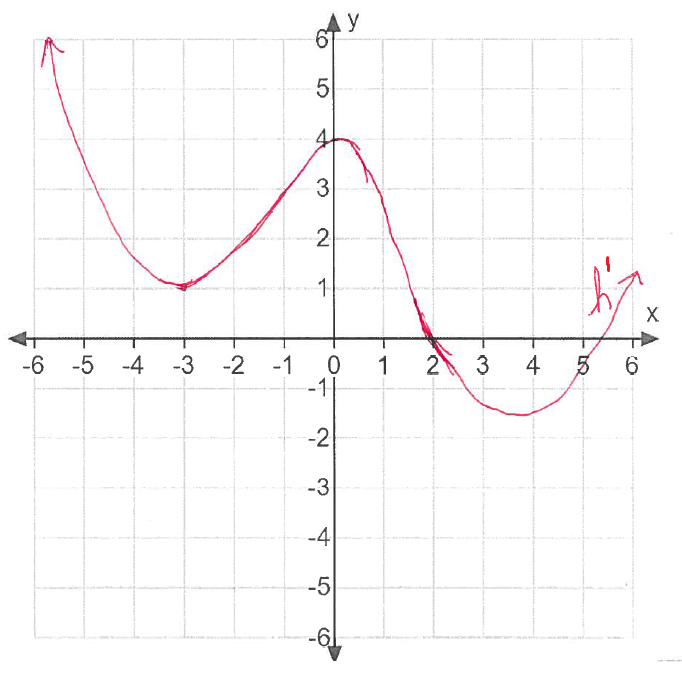
\includegraphics[scale=0.65]{Images/figure1.png}
  \end{image}
  \begin{freeResponse}
    The function is continuous on $[-1,6]$ and differentiable on $(-1,6)$: \\
    hence it satisfies the hypotheses of the Mean Value Theorem.
    \begin{image}
      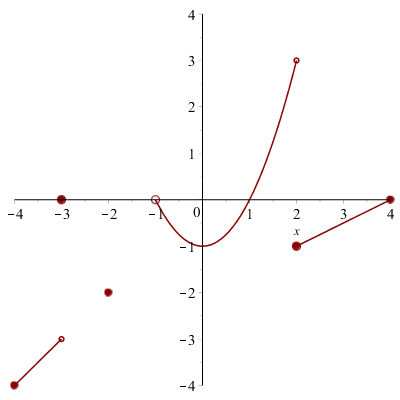
\includegraphics[scale=0.6]{Images/Figure2.png}
    \end{image}
  \end{freeResponse}
\end{problem}

%problem 5
\begin{problem}
  Verify that the given function satisfies the hypotheses of the Mean Value Theorem in the given interval.
  Then algebraically find all numbers $c$ that satisfy the conclusion of the Mean Value Theorem.
  Using the graph provided, label the point(s) $c$ and sketch the secant line and the tangent line at $c$
  $$ f(x) = \frac{x}{x+2} \qquad \text{on } [1,4] $$.
  \begin{image}
    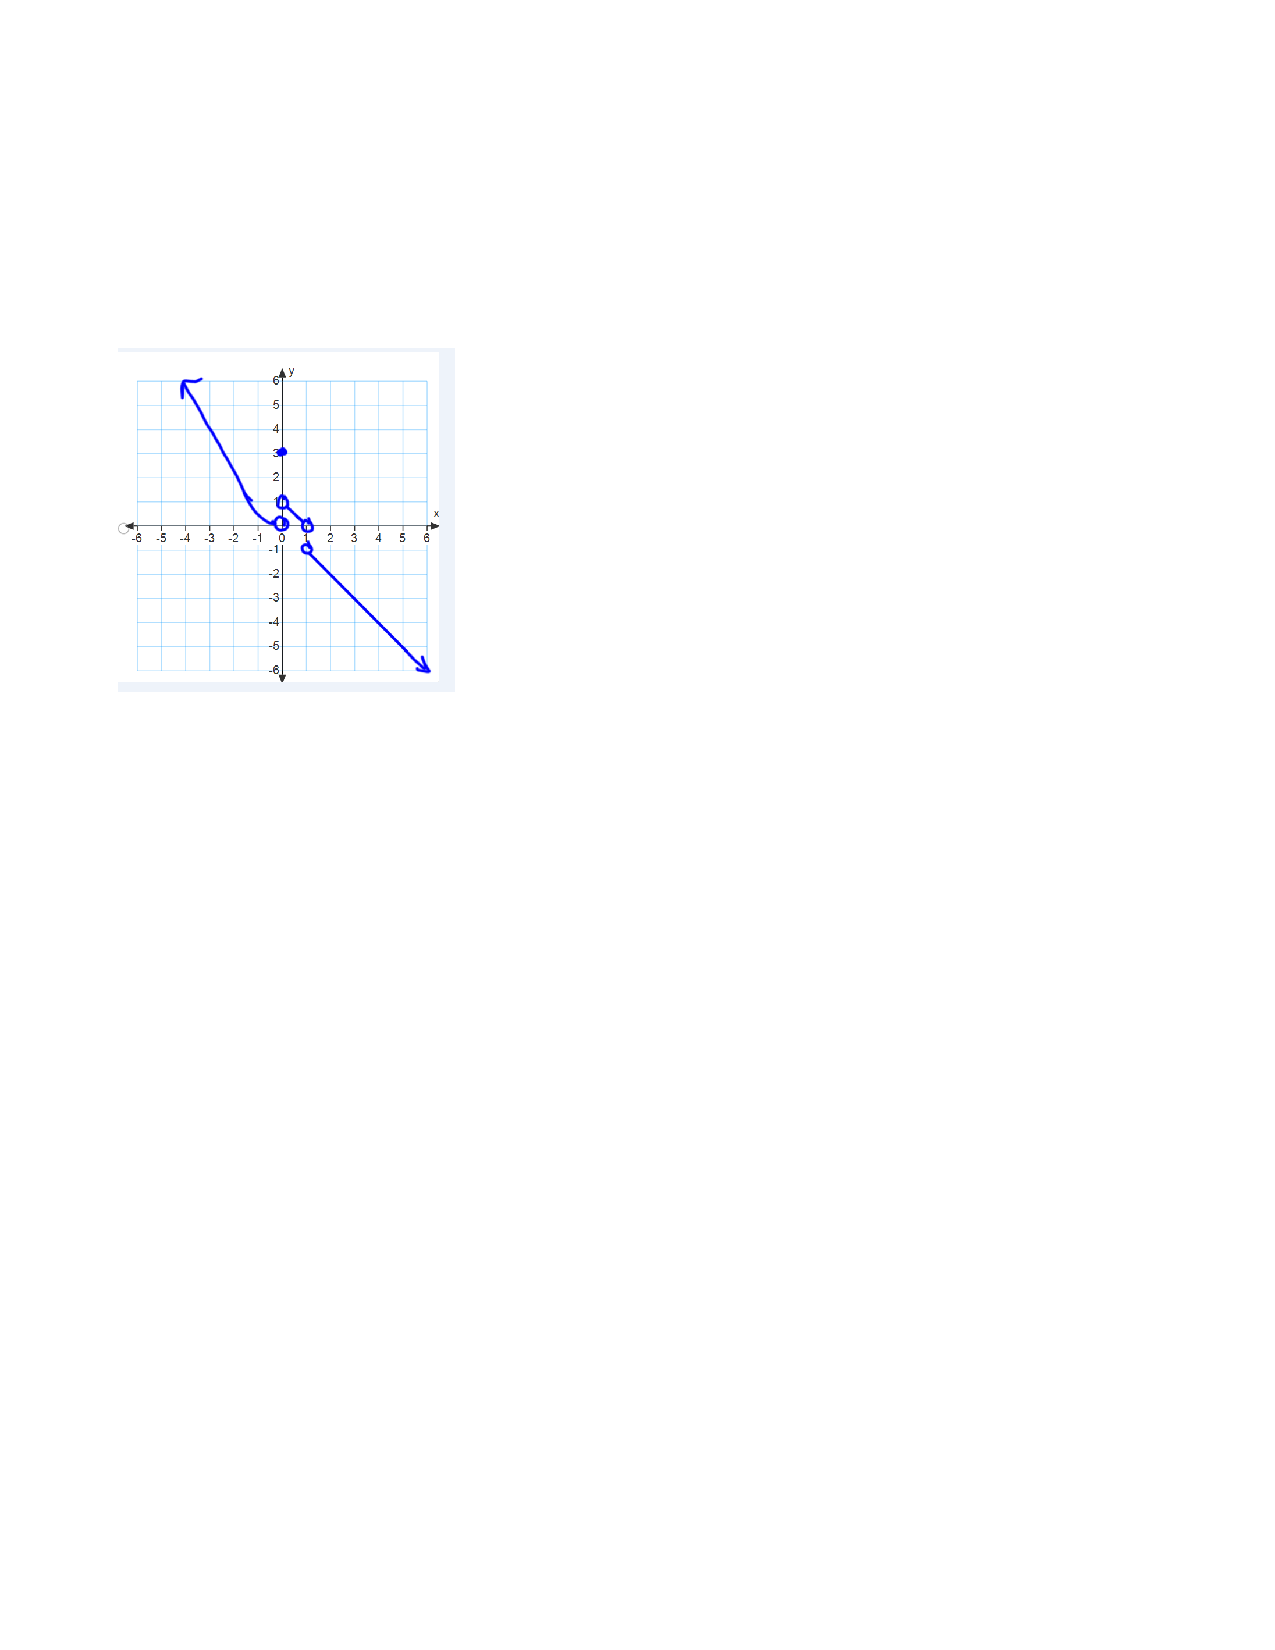
\includegraphics[scale=0.45]{Images/Figure3.png}
  \end{image}
  \begin{freeResponse}
    The function $f(x) = \frac{x}{x+2}$ is continuous on $[1,4]$ and differentiable on $(1,4)$ since it is a rational function, and is therefore continuous and differentiable on its domain.
    Therefore, $f$ satisfies the hypotheses of the Mean Value Theorem.
    We have that
    $$ f'(x) = \frac{(x+2)(1) - x(1)}{(x+2)^2} = \frac{2}{(x+2)^2} $$
    $$ \frac{f(4) - f(1)}{4-1} = \frac{\frac{2}{3} - \frac{1}{3}}{3} = \frac{1}{9} $$
    So we are looking to find all points $c \in (1,4)$ which satisfy that $ f'(c) = \frac{1}{9} $.  So we solve:
    $$ \frac{2}{(c+2)^2} = \frac{1}{9} $$
    $$ (c+2)^2 = 18 $$
    $$ c = \sqrt{18} - 2 = 3\sqrt{2} - 2 $$
    Note that we omitted $-\sqrt{18} - 2$ above because it is not in the interval $(1,4)$.  Therefore, $c = 3\sqrt{2} - 2$.
       \begin{image}
      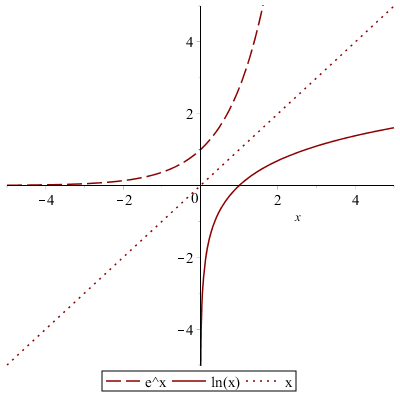
\includegraphics[scale=0.45]{Images/Figure4.png}
    \end{image}
  \end{freeResponse}
\end{problem}

%problem 6
\begin{problem}
  Let $f(x) = (x-3)^{-2}$.
  Show that there is no value $c$ in $(1,4)$ such that $f(4) - f(1) = f^{\prime}(c) (4-1)$.
  Why does this not contradict the Mean Value Theorem?
  \begin{freeResponse}
    First notice that 
    $$f(4)-f(1) = 1^{-2} - (-2)^{-2} = 1-\frac{1}{4} = \frac{3}{4}$$
    and so we are looking for a value $c$ such that 
    $$3 f^\prime (c) = \frac{3}{4} \quad \Longrightarrow \quad f^\prime (c) = \frac{1}{4} $$
    Then since $f'(x) = \frac{-2}{(x-3)^3}$, we can compute:
    $$ f'(c) = \frac{-2}{(c-3)^3} := \frac{1}{4}$$
    $$ (c-3)^3 = - 8 $$
    $$ c = 3 - 2 = 1 $$
    But $1$ is not in the interval $(1,4)$.  This does not contradict the Mean Value Theorem since $f$ is not continuous at $x=3$.

    \begin{image}
      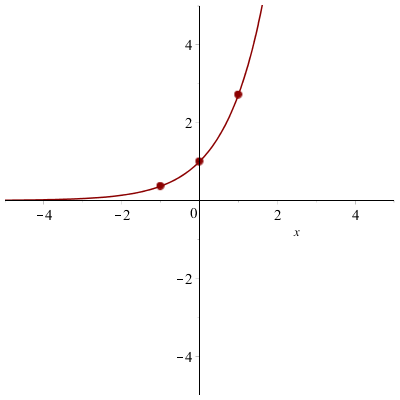
\includegraphics[scale=.65]{Images/Figure5.png}
    \end{image}
  \end{freeResponse}
\end{problem}

%problem7
\begin{problem}
  Two runners start a race at the same time and finish in a tie.
  Prove that at some time during the race they have the same speed.
  (Hint:  Consider the function $h(t)=f(t)-g(t)$, where $f(t)$ and $g(t)$ are the position of the first and second runner at time $t$, respectively.)
  \begin{freeResponse}
    Let $f(t)$ be the position of the first runner at time $t$, and let $g(t)$ be the position of the second runner at time $t$.
    Let $T$ denote the time that the two runners finish the race (which is the same, since they finish in a tie).
    Also, let $h(t) = f(t) - g(t)$.
    Since $h(0) = 0$ and $h(T) = 0$, by Rolle's Theorem there exists some $c$ with $0 < c < T$ such that $h'(c)=0$.
    But since $h^\prime (t) = f^\prime (t) - g^\prime (t)$, we have that $f^\prime (c) = g^\prime (c)$.
    Therefore, the runners have the same speed at time $c$.  

    \begin{image}
      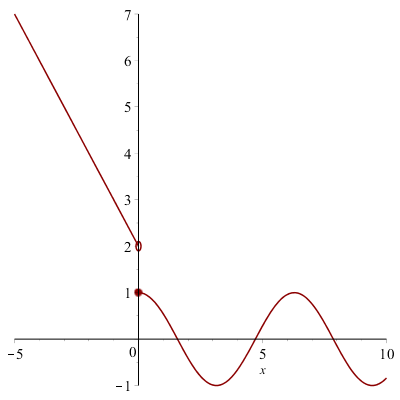
\includegraphics[scale=.45]{Images/Figure6.png}
    \end{image}
  \end{freeResponse}
\end{problem}
\end{document} 
